\begin{frame}[t]{Unidade básica de armazenamento}
    \transboxout[duration=0.5]
    \framesubtitle{Shell - Bits mecânicos}
    \begin{columns}
        \column{.1\textwidth}
        \column{.4\textwidth}

        \begin{figure}[H]
            \centering
            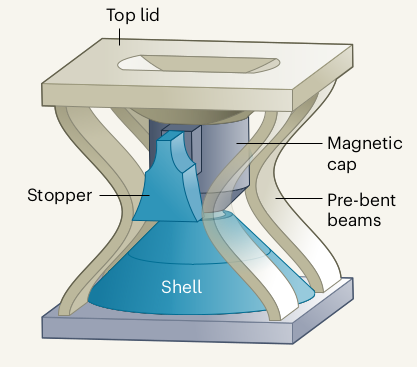
\includegraphics[scale = 0.325]{source/pictures/shell.png}
            \caption{Unidade básica de armazenamento mecânico\cite{coulais2021snappy}.}
            \label{fig:uba}
        \end{figure}

        \column{.6\textwidth}
            \begin{itemize}
                \item Instabilidade de encaixe.
                \item Orientação magnética.
                \item Limitação de movimentação.
            
            \end{itemize}
    \end{columns}
    
    \note[item]{Somente duas posições possuem estabilidade em sua configuração.}
\end{frame}

\begin{frame}[t]{Unidade básica de armazenamento}
    \transboxout[duration=0.5]
    \framesubtitle{Comportamento da estrutura}
    \transboxin[duration=1,direction=30]
    
    \begin{figure}
        \begin{figure}[H]
            \centering
            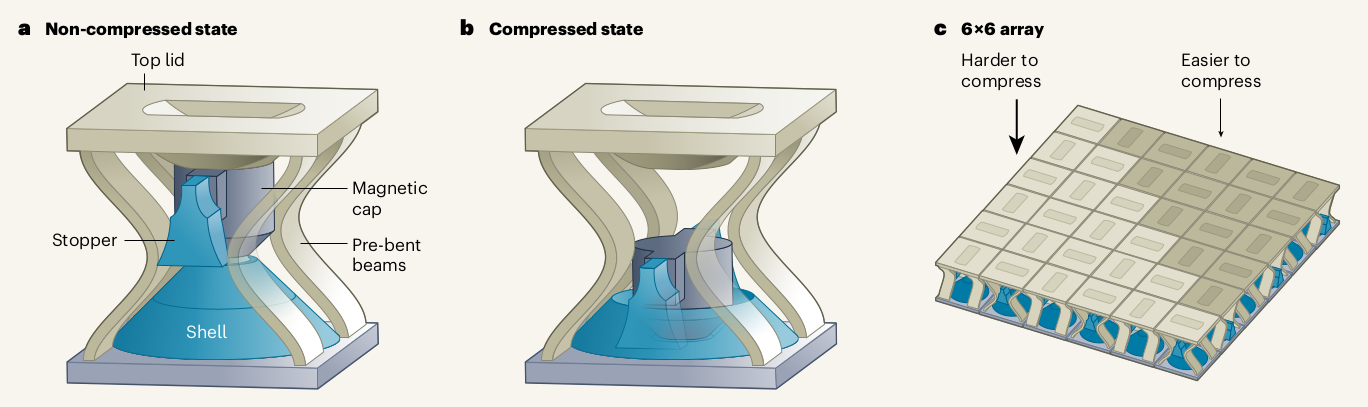
\includegraphics[width = \textwidth]{source/pictures/shell-work.png}
            \caption{Estados da UBA\footnote[1]{Unidade Básica de Armazenamento.}\cite{coulais2021snappy}.}
            \label{fig:uba-states}
        \end{figure}
        %\caption{.}
    \end{figure}
    \small
\end{frame}

\begin{frame}{Processo de gravação}
    \framesubtitle{Em uma unidade básica}
    \centering % Para centralizarmos o vídeo
    \includemedia[
    label=nome_qualquer, % ! Importante para linkar o vídeo ao botão (ver abaixo)
    width=0.6\linewidth, height=0.375\linewidth, % Dimensões
    addresource=./source/movies/record-shell.mp4, % ESTE É O SEU ARQUIVO DE VÍDEO (mesmo dir.)
    transparent, % Opções para que o player tenha transparência
    activate=pageopen, % Se você deseja que o vídeo esteja "carregado" ao abrir a página
    flashvars={
    source=./source/movies/record-shell.mp4
    &loop=true % Se você quer que o vídeo repita automaticamente 
    &scaleMode=letterbox % Manter proporções (dimensionais) do vídeo
    }
    ]{}{VPlayer.swf}
    \vspace{1cm} % Espaçamento entre vídeo e botão
    
    % Agora, você cria o botão para dar play/pause. Neste caso, o botão é apenas a letra "pi".
    
    \mediabutton[
    mediacommand=nome_qualquer:playPause,
    overface=\color{black}{{\strut $\pi$}},
    downface=\color{gray}{{\strut $\pi$}}
    ]{{\strut $\pi$}}
    
    
\end{frame}

\begin{frame}{Processo de gravação}
    \framesubtitle{Em uma unidade básica}
    \centering % Para centralizarmos o vídeo
    \includemedia[
    label=nome_qualquer, % ! Importante para linkar o vídeo ao botão (ver abaixo)
    width=0.6\linewidth, height=0.375\linewidth, % Dimensões
    addresource=./source/movies/recording-array.mp4, % ESTE É O SEU ARQUIVO DE VÍDEO (mesmo dir.)
    transparent, % Opções para que o player tenha transparência
    activate=pageopen, % Se você deseja que o vídeo esteja "carregado" ao abrir a página
    flashvars={
    source=./source/movies/recording-array.mp4
    &loop=true % Se você quer que o vídeo repita automaticamente 
    &scaleMode=letterbox % Manter proporções (dimensionais) do vídeo
    }
    ]{}{VPlayer.swf}
    \vspace{1cm} % Espaçamento entre vídeo e botão
    
    % Agora, você cria o botão para dar play/pause. Neste caso, o botão é apenas a letra "pi".
    
    \mediabutton[
    mediacommand=nome_qualquer:playPause,
    overface=\color{black}{{\strut $\pi$}},
    downface=\color{gray}{{\strut $\pi$}}
    ]{{\strut $\pi$}}
    
    
\end{frame}